
%%%%%%%%%%%%%%%%%%%%%%%%%%%%%%%%%%%%%%%%%%%%%%%%%%%%%%%%%%%%%%%%%%%%%
%% This is a (brief) model paper using the achemso class
%% The document class accepts keyval options, which should include
%% the target journal and optionally the manuscript type.
%%%%%%%%%%%%%%%%%%%%%%%%%%%%%%%%%%%%%%%%%%%%%%%%%%%%%%%%%%%%%%%%%%%%%
\documentclass[journal=jacsat,manuscript=article]{achemso}

%%%%%%%%%%%%%%%%%%%%%%%%%%%%%%%%%%%%%%%%%%%%%%%%%%%%%%%%%%%%%%%%%%%%%
%% Place any additional packages needed here.  Only include packages
%% which are essential, to avoid problems later. Do NOT use any
%% packages which require e-TeX (for example etoolbox): the e-TeX
%% extensions are not currently available on the ACS conversion
%% servers.
%%%%%%%%%%%%%%%%%%%%%%%%%%%%%%%%%%%%%%%%%%%%%%%%%%%%%%%%%%%%%%%%%%%%%
\usepackage[version=3]{mhchem} % Formula subscripts using \ce{}

%%%%%%%%%%%%%%%%%%%%%%%%%%%%%%%%%%%%%%%%%%%%%%%%%%%%%%%%%%%%%%%%%%%%%
%% If issues arise when submitting your manuscript, you may want to
%% un-comment the next line.  This provides information on the
%% version of every file you have used.
%%%%%%%%%%%%%%%%%%%%%%%%%%%%%%%%%%%%%%%%%%%%%%%%%%%%%%%%%%%%%%%%%%%%%
%%\listfiles

%%%%%%%%%%%%%%%%%%%%%%%%%%%%%%%%%%%%%%%%%%%%%%%%%%%%%%%%%%%%%%%%%%%%%
%% Place any additional macros here.  Please use \newcommand* where
%% possible, and avoid layout-changing macros (which are not used
%% when typesetting).
%%%%%%%%%%%%%%%%%%%%%%%%%%%%%%%%%%%%%%%%%%%%%%%%%%%%%%%%%%%%%%%%%%%%%
\newcommand*\mycommand[1]{\texttt{\emph{#1}}}

%%%%%%%%%%%%%%%%%%%%%%%%%%%%%%%%%%%%%%%%%%%%%%%%%%%%%%%%%%%%%%%%%%%%%
%% Meta-data block
%% ---------------
%% Each author should be given as a separate \author command.
%%
%% Corresponding authors should have an e-mail given after the author
%% name as an \email command. Phone and fax numbers can be given
%% using \phone and \fax, respectively; this information is optional.
%%
%% The affiliation of authors is given after the authors; each
%% \affiliation command applies to all preceding authors not already
%% assigned an affiliation.
%%
%% The affiliation takes an option argument for the short name.  This
%% will typically be something like "University of Somewhere".
%%
%% The \altaffiliation macro should be used for new address, etc.
%% On the other hand, \alsoaffiliation is used on a per author basis
%% when authors are associated with multiple institutions.
%%%%%%%%%%%%%%%%%%%%%%%%%%%%%%%%%%%%%%%%%%%%%%%%%%%%%%%%%%%%%%%%%%%%%
\author{Hongjian Li}
\email{jackyleehongjian@gmail.com}
\author{Kwong-Sak Leung}
\author{Man-Hon Wong}
\affiliation[Chinese University of Hong Kong]
{Department of Computer Science and Engineering, Chinese University of Hong Kong, Shatin, New Territories, Hong Kong}
\author{Pedro J. Ballester}
\email{pedro.ballester@ebi.ac.uk}
\affiliation[European Bioinformatics Institute]
{European Bioinformatics Institute, Wellcome Trust Genome Campus, Hinxton, Cambridge - CB10 1SD, UK}

%%%%%%%%%%%%%%%%%%%%%%%%%%%%%%%%%%%%%%%%%%%%%%%%%%%%%%%%%%%%%%%%%%%%%
%% The document title should be given as usual. Some journals require
%% a running title from the author: this should be supplied as an
%% optional argument to \title.
%%%%%%%%%%%%%%%%%%%%%%%%%%%%%%%%%%%%%%%%%%%%%%%%%%%%%%%%%%%%%%%%%%%%%
\title[RF::Cyscore]{Improving Protein-Ligand Binding Affinity Prediction by Substituting Random Forest for Multiple Linear Regression: Using Cyscore as an Example}

%%%%%%%%%%%%%%%%%%%%%%%%%%%%%%%%%%%%%%%%%%%%%%%%%%%%%%%%%%%%%%%%%%%%%
%% Some journals require a list of abbreviations or keywords to be
%% supplied. These should be set up here, and will be printed after
%% the title and author information, if needed.
%%%%%%%%%%%%%%%%%%%%%%%%%%%%%%%%%%%%%%%%%%%%%%%%%%%%%%%%%%%%%%%%%%%%%
\abbreviations{MLR,RF}
\keywords{Molecular docking, binding affinity, machine learning}

%%%%%%%%%%%%%%%%%%%%%%%%%%%%%%%%%%%%%%%%%%%%%%%%%%%%%%%%%%%%%%%%%%%%%
%% The manuscript does not need to include \maketitle, which is
%% executed automatically.
%%%%%%%%%%%%%%%%%%%%%%%%%%%%%%%%%%%%%%%%%%%%%%%%%%%%%%%%%%%%%%%%%%%%%
\begin{document}

%%%%%%%%%%%%%%%%%%%%%%%%%%%%%%%%%%%%%%%%%%%%%%%%%%%%%%%%%%%%%%%%%%%%%
%% The "tocentry" environment can be used to create an entry for the
%% graphical table of contents. It is given here as some journals
%% require that it is printed as part of the abstract page. It will
%% be automatically moved as appropriate.
%%%%%%%%%%%%%%%%%%%%%%%%%%%%%%%%%%%%%%%%%%%%%%%%%%%%%%%%%%%%%%%%%%%%%
\begin{tocentry}

Some journals require a graphical entry for the Table of Contents.
This should be laid out ``print ready'' so that the sizing of the
text is correct.

Inside the \texttt{tocentry} environment, the font used is Helvetica
8\,pt, as required by \emph{Journal of the American Chemical
Society}.

The surrounding frame is 9\,cm by 3.5\,cm, which is the maximum
permitted for  \emph{Journal of the American Chemical Society}
graphical table of content entries. The box will not resize if the
content is too big: instead it will overflow the edge of the box.

This box and the associated title will always be printed on a
separate page at the end of the document.

\end{tocentry}

%%%%%%%%%%%%%%%%%%%%%%%%%%%%%%%%%%%%%%%%%%%%%%%%%%%%%%%%%%%%%%%%%%%%%
%% The abstract environment will automatically gobble the contents
%% if an abstract is not used by the target journal.
%%%%%%%%%%%%%%%%%%%%%%%%%%%%%%%%%%%%%%%%%%%%%%%%%%%%%%%%%%%%%%%%%%%%%
\begin{abstract}



\end{abstract}

%%%%%%%%%%%%%%%%%%%%%%%%%%%%%%%%%%%%%%%%%%%%%%%%%%%%%%%%%%%%%%%%%%%%%
%% Start the main part of the manuscript here.
%%%%%%%%%%%%%%%%%%%%%%%%%%%%%%%%%%%%%%%%%%%%%%%%%%%%%%%%%%%%%%%%%%%%%
\section{Introduction}

Protein-ligand docking is a structural bioinformatic method that predicts how a ligand binds to a target protein and their binding affinity. Hence docking is useful in elaborating intermolecular interactions and enhancing the potency and selectivity of binding in subsequent phases of the modern drug discovery process. Docking has a wide variety of pragmatic and successful applications in structure-based virtual screening, drug repurposing, lead compound optimization, protein cavity idenitfication, protein function prediction, etc.

Operationally speaking, docking consists of two major steps: predicting the position, orientation and conformation of a ligand when docked to the protein’s binding pocket, and predicting their binding strength. The former step is known as pose generation, and the latter is known as scoring. State-of-the-art docking methods, such as AutoDock Vina \cite{595} and idock \cite{1153}, have managed to cope with the pose generation subproblem with a redocking success rate of over 50\% \cite{1362} on both the PDBbind \cite{529,530} and the CSAR \cite{857,960} benchmarks. Therefore the single most critical limitation of docking is the traditionally low accuracy of the scoring functions.

Classical scoring functions assume a fixed functional form for the relationship between the numerical features that describe the protein-ligand complex and its predicted binding affinity. Such functional form is typically inspired by some sorts of established chemistry theories, and is often additive. The overall binding affinity is calculated as a weighted sum of several physically meaningful terms, while their coefficients are derived from regression analysis on experimental data. Cyscore \cite{1372}, a recently published empirical scoring function, is an example of classical scoring functions.

Cyscore assumes that the overall protein-ligand binding free energy can be decomposed into four terms: hydrophobic free energy, van der Waals interaction energy, hydrogen bond interaction energy and ligand's conformational entropy (Eq. \ref{eqn:cyscore}). $k_h$, $k_v$, $k_b$ and $k_e$ are the coefficients, which were obtained by standard least-square multivariate linear regression (MLR) on a training set of 247 complexes carefully selected from PDBbind v2012. Cyscore mainly focuses on improving the prediction of hydrophobic free energy by using a novel curvature-dependent surface-area model, which is able to distinguish convex, planar and concave surface in hydrophobic free energy calculation.

\begin{equation}
\Delta G_{bind} = k_h\Delta G_{hydrophobic} + k_v\Delta G_{vdw} + k_b\Delta G_{hbond} + k_e\Delta G_{entropy}
\label{eqn:cyscore}
\end{equation}

In addition to classical scoring functions, recent years have seen a growing number of new developments of machine-learning scoring functions, with RF-Score \cite{564} being one of the representatives. RF-Score, as its name suggests, uses Random Forest (RF) \cite{1309} to implicitly learn the functional form in an entirely data-driven manner, and thus circumvents the modeling assumption of classical scoring functions. RF-Score was shown to outperform 16 classical scoring functions when evaluated on the common PDBbind v2007 benchmark \cite{564}. Despite being a recent development, RF-Score has already been successfully used to discover a large number of innovative binders against antibacterial DHQase2 targets \cite{1281}. For the purpose of prospective virtual screening, RF-Score has now been incorporated into istar \cite{1362}, a user-friendly large-scale docking service available at http://istar.cse.cuhk.edu.hk/idock.

In this study we compare the prediction performance of MLR and RF in various contexts, and investigate the conditions of substituting RF for MLR.

\section{Methods}

2 models, 3 feature sources: Cyscore, AutoDock Vina and RF-Score.

MLR vs RF were compared as two regression models.

by analysing how their performances improve with the increase of structural and binding data used for training.

This section introduces three SFs building upon Autodock Vina, two benchmarks to evaluate performance of these SFs and the performance metrics that will be used to this end.

\subsection{Multiple Linear Regression (MLR)}

Cyscore v1.1.2

\subsection{Random Forset (RF)}

A RF is an ensemble of many different decision trees randomly generated from the same training data \cite{1309}. Instead of using all features, RF selects the best data split at each node of the tree from a typically small number (mtry) of randomly chosen features. In regression problems, the RF prediction is given by arithmetic mean of all the individual tree predictions in the forest. Here we built a RF model with the six Vina features using the default number of trees (500) and values of the mtry control parameter from 1 to all 6 features. The selected model will be that with the mtry value providing the lowest RMSE on a subset of training data known as the Out-of-Bag (OOB) data. Further details on RF model building in this context can be found in \cite{564}.

one single seed, no significant difference

additional features: AutoDock Vina \cite{595}, RF-Score \cite{564}

Vina’s score consists of 6 features, which are gauss1, gauss2, repulsion, hydrophobic effect and hydrogen bonding. Detail can be found in \cite{1362}.

RF-Score features are defined as the occurrence count of intermolecular contacts between two elemental atom types. Protein (C,N,O,S) and ligand (C, N, O, S, P, F, Cl, Br, I) Atom types are selected so as to generate features that are as dense as possible, while considering all the heavy atom types commonly observed in protein-ligand complexes.

\subsection{PDBbind v2007 and v2012 benchmarks}

The PDBbind v2007 benchmark is based on the 2007 version of the PDBbind database, which contains a particularly diverse collection of protein-ligand complexes (1300 protein-ligand complexes with their corresponding binding affinities), assembled through a systematic mining of the entire PDB. The PDBbind benchmark essentially consists of testing the predictions of SFs on the 2007 core set, which comprises 195 diverse complexes with measured binding affinities spanning more than 12 orders of magnitude, while training in the remaining 1105 complexes in the refined set. In this way, a set of protein-ligand complexes with measured binding affinity can be processed to give two non-overlapping data sets.

The PDBbind benchmark is arguably the most widely-used for binding affinity prediction. This benchmark has the advantage of permitting a direct comparison against the performance of 16 classical SFs on the same test set \cite{1313}. Using a predefined training and test sets, where other SFs had previously been tested, has the advantage of minimising the risk of using a benchmark complementary to the presented SF.

new training set: Cyscore used 247 complexes selected from the PDBbind v2012 refined set using certain criteria.

Two test sets: core07 and core12.

The PDBbind v2012 dataset contains a diverse collection of experimentally determined structures carefully selected from PDB (Protein Data Bank) \cite{540,537}. For each complex, the experimental binding affinity (either dissociation constant $K_d$, inhibition constant $K_i$, or half maximal inhibitory concentration $IC_{50}$) is manually collected from its primary literature reference, thus resulting in the general set of 9,308 complexes, with 7,121 being protein-ligand complexes. Out of them, the complexes with a resolution of 2.5\AA\ or better, with known $K_d$ or $K_i$ values, and with ligand containing merely the common heavy atoms (i.e. C, N, O, F, P, S, Cl, Br, I) are filtered to constitute the refined set of 2,897 complexes. These complexes are then clustered by protein sequence similarity using BLAST at a cutoff of 90\%, and for each of the 67 resulting clusters with at least five complexes, the three complexes with the highest, median and lowest binding affinity are selected to constitute the core set of 201 complexes, whose experimental binding affinity spans 10 $pK_d$ or $pK_i$ units.

The overlaps between training and test sets = 0. |refined12 U core12| = 28

\subsection{PDBbind v2013 blind test}

We propose a new benchmark mimicking a blind test in order to study how performance varies with training data set size. The test set will be all the structures in the 2013 release of the PDBbind refined set that were not already in the 2012 release. It resulted in 382 protein-ligand complexes. To account for the structural and binding data available in the public domain at four previous times, we will use as training sets four previous PDBbind releases (these were selected so that there is approximately the same number of complexes between consecutive releases). In this way, we have not control on the composition of each training set or test set, while the benchmark is conducted as a blind test in that we use all the data available on a certain year to predict the binding affinities of 2013 complexes as if these had not been measured yet. By construction, there are no complexes in common between the test set and any of the training sets. 

The four training sets are the refined sets of PDBbind v2002 (N=792), v2007 (N=1300), v2010 (N=2059) and v2012 (N=2897).

\subsection{Performance Measures}

We quantified the prediction accuracy through standard deviation (SD) in linear correlation, Pearson's correlation coefficient (Rp) and Spearman's correlation coefficient (Rs), three commonly used criteria for binding affinity prediction.

\begin{equation}
SD = \sqrt{\frac{1}{N-2}\sum_{n=1}^N(y^{(n)}-(a+bp^{(n)})^2}
\label{eqn:sd}
\end{equation}

\begin{equation}
R_p = \frac{N\sum_{n=1}^Np^{(n)}y^{(n)}-\sum_{n=1}^Np^{(n)}\sum_{n=1}^Ny^{(n)}}{N}
\label{eqn:rp}
\end{equation}

Note that these three measures are invariant under linear transformations (e.g. changing the intercept value obtained by linear regression), so they are mainly used for comparative purpose. In some applications the ultimate goal of scoring functions is to report an absolute binding affinity value as close to the measured value as possible. Hence we propose a more realistic measure, RMSE, which is calculated between measured binding affinities and the predicted ones without in a linear correlation.

\section{Results and discussion}

preamble

\subsection{For MLR, more training data lead to worse prediction performance}

\begin{table}
\caption{Prediction performance of MLR}
\label{tbl:performance}
\begin{tabular}{rrrrrrrr}
\hline
model & x & trn & tst & RMSE & SD & Rp & Rs\\
MLR & 2 &  247 & 195 & 1.88 & 1.89 & 0.612 & 0.637\\
MLR & 2 & 1105 & 195 & 1.96 & 1.92 & 0.594 & 0.632\\
MLR & 2 & 2280 & 195 & 2.03 & 1.96 & 0.569 & 0.611\\
MLR & 4 &  247 & 195 & 1.80 & 1.79 & 0.660 & 0.687\\
MLR & 4 & 1105 & 195 & 1.87 & 1.82 & 0.649 & 0.681\\
MLR & 4 & 2280 & 195 & 1.93 & 1.83 & 0.643 & 0.676\\
MLR & 2 &  247 & 201 & 1.94 & 1.94 & 0.600 & 0.607\\
MLR & 2 & 1105 & 201 & 2.02 & 1.97 & 0.585 & 0.587\\
MLR & 2 & 2280 & 201 & 2.08 & 2.01 & 0.563 & 0.566\\
MLR & 4 &  247 & 201 & 1.88 & 1.89 & 0.630 & 0.639\\
MLR & 4 & 1105 & 201 & 1.95 & 1.92 & 0.610 & 0.625\\
MLR & 4 & 2280 & 201 & 2.00 & 1.95 & 0.596 & 0.608\\
\hline
\end{tabular}
\end{table}

\begin{figure}
\minipage{0.33\textwidth}
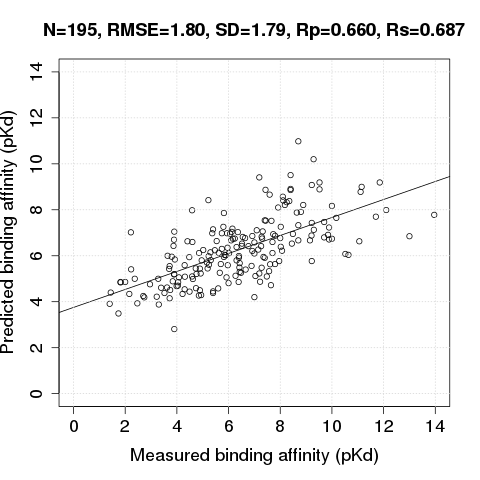
\includegraphics[width=1.4\linewidth,natwidth=480,natheight=480]{../rfcyscore/x4/mlr/trn-247-tst-195-yp.png}
\endminipage\hfill
\minipage{0.33\textwidth}
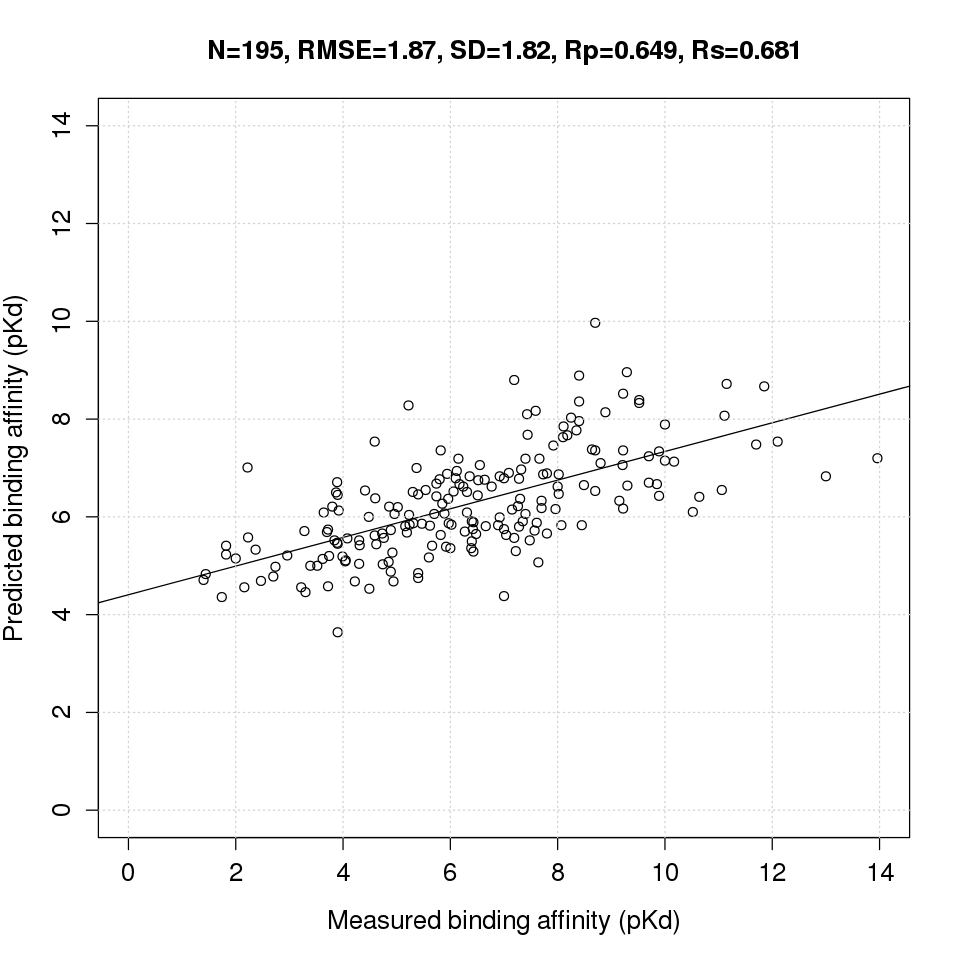
\includegraphics[width=1.4\linewidth,natwidth=480,natheight=480]{../rfcyscore/x4/mlr/trn-1105-tst-195-yp.png}
\endminipage\hfill
\minipage{0.33\textwidth}%
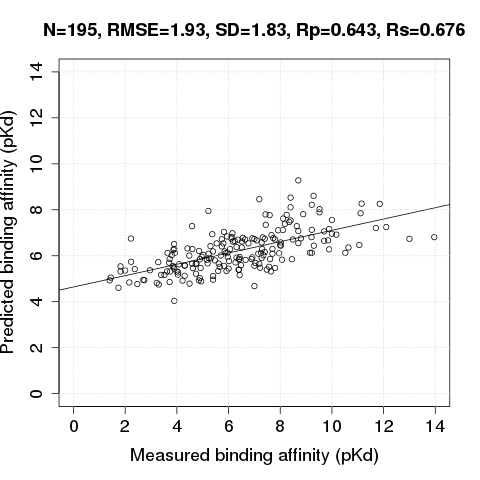
\includegraphics[width=1.4\linewidth,natwidth=480,natheight=480]{../rfcyscore/x4/mlr/trn-2280-tst-195-yp.png}
\endminipage
\caption{MLR performance on PDBbind v2007 core set (N = 195).}
\label{fig:mlr-tst-195}
\end{figure}

Conclusion: For MLR, more training data lead to worse prediction performance. Better to select fewer training samples, but of high quality, like Cyscore did.
improvements with data set size can only be gain with the appropriate regression model anyway.

\subsection{refined07\\core07 not a good benchmark}

Same cluster (protein family)

Conclusion: refined07\\core07 not a good benchmark.
The superior performance of RF-Score was highlighted by (Kramer and Gedeck, 2010), who nevertheless attribute it to the characteristics of the most widely-used benchmark. \cite{774}


\subsection{Machine-learning SFs assimilate data better than Empirical SFs}

Figure 2 shows their performance on PDBbind benchmark, with RF::VinaElem greatly improving Vina by -0.90 in RMSE, -0.57 in SD, +0.249 in Rp and +0.190 in Rs.
RF is capable of effectively exploiting a more comprehensive set of structural features.
not only the difference in performance is substantial but grows as more data is available for training, thus increasing the importance of using RF.

\subsection{Machine-learning SFs are remarkably more accurate than Empirical SFs}

\begin{table}
\caption{Pearson's correlation coefficient $R_p$, Spearman's correlation coefficient $R_s$ and standard deviation $SD$ of the difference between predicted and experimental binding affinity on PDBbind v2007 core set ($N$ = 195). The scoring functions are sorted in the descending order of $R_p$. RF-Score, AutoDock Vina and idock rank 1st, 7th and 8th respectively in terms of Pearson's correlation coefficient $R_p$. RF-Score, ID-Score, SVR-Score and X-Score are the only scoring functions whose training set do not overlap with the PDBbind v2007 core set. The statistics for AutoDock Vina and idock are reported in this study and the statistics for the other 19 scoring functions are collected from \cite{1313,564,1305,1295}.}
\label{tbl:sf}
\begin{tabular}{lrrr}
\hline
Scoring function & $R_p$ & $R_s$ & $SD$\\
\hline
RF-Score & 0.774 & 0.762 & 1.59\\
ID-Score & 0.753 & 0.779 & 1.63\\
SVR-Score & 0.726 & 0.739 & 1.70\\
X-Score::HMScore & 0.644 & 0.705 & 1.83\\
DrugScoreCSD & 0.569 & 0.627 & 1.96\\
SYBYL::ChemScore & 0.555 & 0.585 & 1.98\\
AutoDock Vina & 0.554 & 0.608 & 1.98\\
idock & 0.546 & 0.612 & 1.99\\
DS::PLP1 & 0.545 & 0.588 & 2.00\\
GOLD::ASP & 0.534 & 0.577 & 2.02\\
SYBYL::G-Score & 0.492 & 0.536 & 2.08\\
DS::LUDI3 & 0.487 & 0.478 & 2.09\\
DS::LigScore2 & 0.464 & 0.507 & 2.12\\
GlideScore-XP & 0.457 & 0.435 & 2.14\\
DS::PMF & 0.445 & 0.448 & 2.14\\
GOLD::ChemScore & 0.441 & 0.452 & 2.15\\
SYBYL::D-Score & 0.392 & 0.447 & 2.19\\
DS::Jain & 0.316 & 0.346 & 2.24\\
GOLD::GoldScore & 0.295 & 0.322 & 2.29\\
SYBYL::PMF-Score & 0.268 & 0.273 & 2.29\\
SYBYL::F-Score & 0.216 & 0.243 & 2.35\\
    \hline
  \end{tabular}
\end{table}

16 classical SFs on core07 \cite{1313}

\subsection{Cyscore feature usefulness}

Compare x42 and x46

\section{Conclusions}

Machine-learning scoring functions are fundamentally different from classical ones because of not imposing a functional form on the relationship between structural and binding data.
Same training set, same test set, same featuers lead to same applicability domain when it comes to binding affinity prediction.
the superior performance of machine-learning SFs comes exclusively from the avoidance of the assumed functional form of classical SFs. By fixing the remaining design variables (i.e. using the same features, training set and test set), any performance difference must necessarily come from the choice of regression model. Moreover, in this case the used training data and features are identical, so will be the domain of applicability of the resulting SFs. 

%%%%%%%%%%%%%%%%%%%%%%%%%%%%%%%%%%%%%%%%%%%%%%%%%%%%%%%%%%%%%%%%%%%%%
%% The "Acknowledgement" section can be given in all manuscript
%% classes.  This should be given within the "acknowledgement"
%% environment, which will make the correct section or running title.
%%%%%%%%%%%%%%%%%%%%%%%%%%%%%%%%%%%%%%%%%%%%%%%%%%%%%%%%%%%%%%%%%%%%%
\begin{acknowledgement}

We gratefully acknowledge the Direct Grant from the Chinese University of Hong Kong, the GRF Grant (Project No. 2150764) from the Research Grants Council of Hong Kong SAR, and the Medical Research Council for a Methodology Research Fellowship (Grant No. G0902106, awarded to P.J.B.). We also thank Yang Cao for helping us to reproduce the Cyscore results.

\end{acknowledgement}

%%%%%%%%%%%%%%%%%%%%%%%%%%%%%%%%%%%%%%%%%%%%%%%%%%%%%%%%%%%%%%%%%%%%%
%% The same is true for Supporting Information, which should use the
%% suppinfo environment.
%%%%%%%%%%%%%%%%%%%%%%%%%%%%%%%%%%%%%%%%%%%%%%%%%%%%%%%%%%%%%%%%%%%%%
\begin{suppinfo}



\end{suppinfo}

%%%%%%%%%%%%%%%%%%%%%%%%%%%%%%%%%%%%%%%%%%%%%%%%%%%%%%%%%%%%%%%%%%%%%
%% The appropriate \bibliography command should be placed here.
%% Notice that the class file automatically sets \bibliographystyle
%% and also names the section correctly.
%%%%%%%%%%%%%%%%%%%%%%%%%%%%%%%%%%%%%%%%%%%%%%%%%%%%%%%%%%%%%%%%%%%%%
\bibliography{../refworks}

\end{document}
